\documentclass{article}
\usepackage{graphicx}
\usepackage[margin=0.5in]{geometry}
\usepackage{listings}
\usepackage{color}
\usepackage[usenames,dvipsnames,svgnames,table]{xcolor}

\lstset{
	keywordstyle=\color{red},
	stringstyle=\color{blue},
	tabsize=2,
}

\title{Homework 09 - Transcript-Summary-Conclusion Table \& Appendix}
\author{Andrew Carter and Beryl Egerter}

\begin{document}
\maketitle

\section{Transcript-Summary-Conclusion Table}
\subsection{A note on formatting}
Following are annotated transcripts of ACBE4Q1, ACBE3Q1, ACBE3Q4, and ACBE1Q3. The assignment asks for these in a table format. Due to the wordy nature of the transcripts and the conclusions (and partially the summaries), we found the table format which restricts the width of each of these categories to less than a third of the page extremely cramped and almost impossible to read. In the interest of readability we have provided these in a format of: \\
\textit{[time] \\
Speaker:} \\
\hspace*{1em} \textit{transcript} \\
\textbf{Context}: any context required \\
\textbf{Summary}: brief summary of corresponding transcript \\
\textbf{Conclusions}: conclusions drawn from corresponding transcript 

\subsection{High Level Points}
The high level points we are trying to make with these transcripts are:
\begin{itemize}
  \item (ACBE4Q1) Execution order appears to work better for the evaluation questions we have provided. Even by starting using a different method, a participant ended up executing the code instead.
  \item (ACBE3Q1 \& ACBE3Q4)The right method can help a student move past concepts they are not familiar with. While evaluating, a student used execution order which helped him understand a concept, and switching to top down let him ignore a large portion of the code and clear up some misunderstandings.
  \item (ACBE1Q3) Top down order on a debugging question while not understanding many concepts used in the code can lead to someone forgetting the question.
\end{itemize}

\subsection{A note on context}
In the context of each segment of transcript, line numbers are referred to. These line numbers correspond to line numbers of code within the Appendix (Section 2 of this document). Also used are figures which are scanned copies of the paper that the students wrote on during the interviews. The figures follow the annotated transcripts as Section 1.5 of this document.

\newpage
\subsection{remove this page and put in google doc pages here instead}
\newpage
\subsection{Figures}
Fig 1. ACBE1Q3 \\
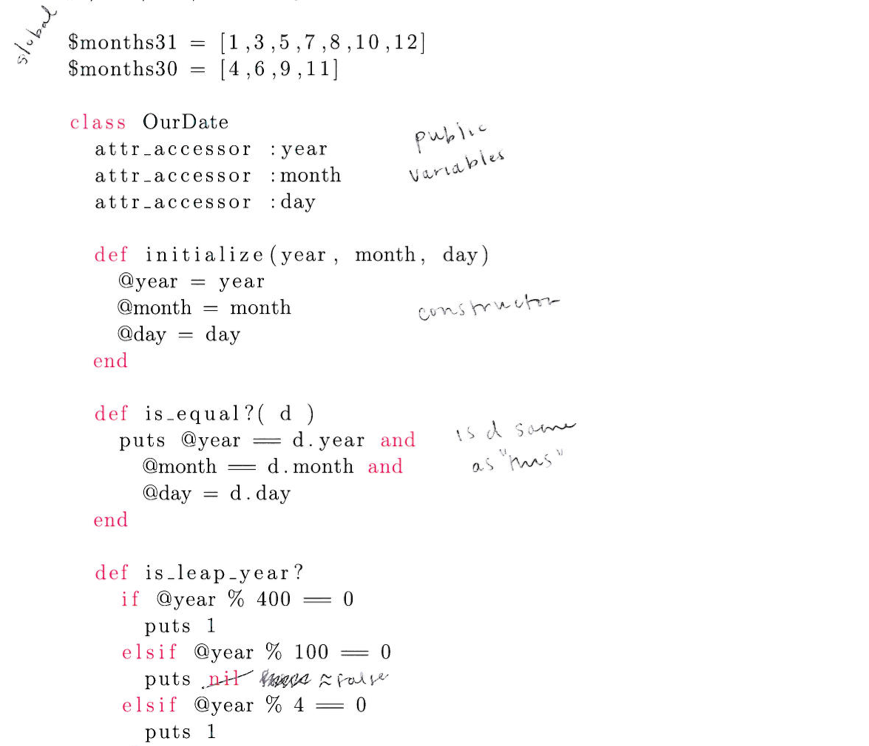
\includegraphics[scale=0.7]{ACBE1Q3.png}
\newpage
Fig 2. ACBE4Q1 \\
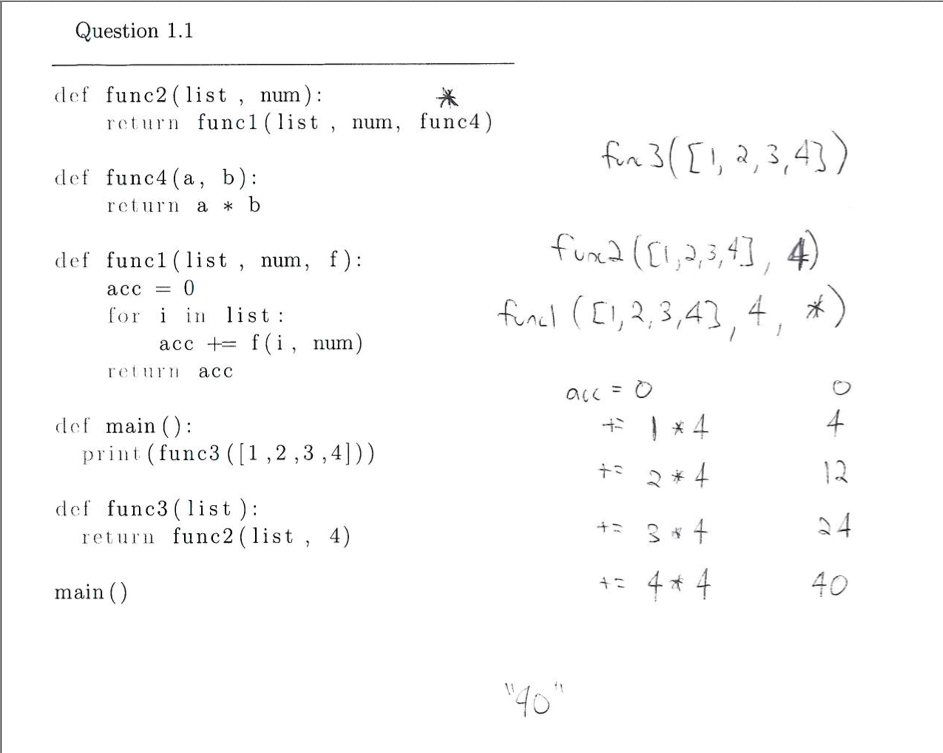
\includegraphics[scale=0.6]{ACBE4Q1.png}
\newpage
Fig 3. ACBE3Q4 \\
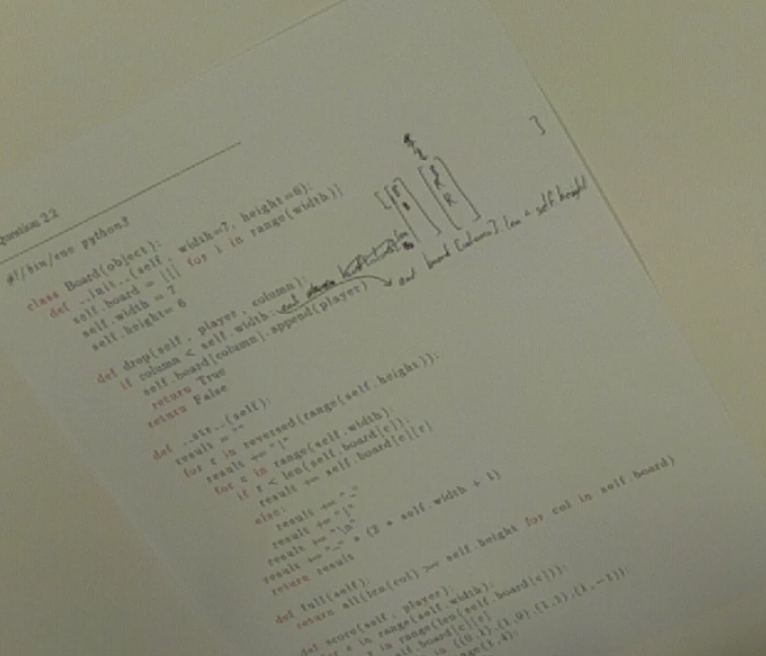
\includegraphics[scale=0.7]{ACBE3Q4.png}
\newpage
\section{Appendix}
\subsection{Interview Question 1}
Code given to participants did not include line numbers. \\
Code given to ACBE1, ACBE2, and ACBE3 was in color. Code given to ACBE4 was in grayscale. \\
Verbal prompt was given before handing code to participant: \\
"For this question we would like you to familiarize yourself with some Python code. Please explain to us what you think this code does." \\
\line(1,0){300}
\begin{lstlisting}[language=python]
0		def func2(list, num):
1			return func1(list, num, func4)
2
3		def func4(a, b):
4			return a * b
5
6		def func1(list, num, f):
7			acc = 0
8			for i in list:
9					acc += f(i, num)
10		return acc
11
12	def main():
13		print(func3([1,2,3,4]))
14
15	def func3(list):
16		return func2(list, 4)
17
18	main()

\end{lstlisting}
\newpage
\subsection{Interview Question 2}
Code given to participants did not include line numbers. \\
Code given to ACBE1, ACBE2, and ACBE3 was in color. Code given to ACBE4 was in grayscale. \\
Verbal prompt was given before handing code to participant: \\
"For this question, we would like you to again familiarize yourself with some Python code. Please explain to us what you think this code does. " \\


\line(1,0){300}
\begin{lstlisting}[language=python]
0		def function50(i, L):
1			return L[i+2]
2
3		def function37(L):
4			return [L[-1]]+L
5
6		def function52(i):
7			return function4() * i
8
9		def function1(j, k):
10		return (j + k) * function52(1)
11
12	def function4():
13		return 3
14
15	def function188(L):
16		return function37(L)+[function50(2, L)]
17
18	def function0():
19		return function188([1,2,3,4,5,6,7,8,9])[function1(0,1)]
20
21	x = function0()
22	print x

\end{lstlisting}

\newpage
\subsection{Interview Question 3}
Code given to participants did not include line numbers. \\
Code given to ACBE1, ACBE2, and ACBE3 was in color. Code given to ACBE4 was in grayscale. 
Code given to ACBE1 and ACBE2 had double equals signs that were joined together. Code given to ACBE3 and ACBE4 had spaces between the equals signs. \\
Verbal prompt was given before handing code to participant: \\
"For this question we would like to have you look at some code in the programming language Ruby. This is the scenario: A coworker recently left on vacation and left two files behind. One of those files is a Date class and your boss wasn't sure if the coworker had finished including leap year support. Your boss would like you to make sure it is supported." \\
\line(1,0){300} \\
File 1: \\
\begin{lstlisting}[language=ruby]
0	#!/usr/bin/ruby
1	
2	load "ourdate.rb"
3	
4	d = OurDate.new(2011,1,4)
5	print "#{d.what_day}"
6	print "We started writing this file today.\n"
7	d.forward_time(365)
8	print "We are almost done now.\n"
9	print "#{d.what_day}"

\end{lstlisting} 
\vspace{1cm} File 2
\begin{lstlisting}[language=ruby]
0		#!/usr/bin/env ruby
1
2		$months31 = [1,3,5,7,8,10,12]
3		$months30 = [4,6,9,11]
4	
5		class OurDate
6			attr_accessor :year
7			attr_accessor :month
8			attr_accessor :day
9	
10		def initialize(year, month, day)
11			@year = year
12			@month = month
13			@day = day
14		end
15
16		def is_equal?( d )
17			puts @year = = d.year and 
18				@month = = d.month and 
19				@day = d.day
20		end
21
22		def is_leap_year?
23			if @year % 400 = = 0
24				puts true
25			elsif @year % 100 = = 0
26				puts false
27			elsif @year % 4 = = 0
28				puts true
29			else
30				puts false
31			end
32		end
33
34		def check_month
35			if @month = = 13
36				@month = 1
37				@year = @year + 1
38			elsif @month = = 0
39				@month = 12
40				@year = @year - 1
41			end
42		end
43
44		def tomorrow
45			@day = @day + 1
46			if @day > 31
47				for i in $months31
48					if @month = = i
49						@day = 1
50						@month = @month + 1
51						check_month
52					end
53				end
54			elsif @day > 30
55				for i in $months30
56					if @month = = i
57						@day = 1
58						@month = @month + 1
59						check_month
60					end
61				end
62			elsif @day > 28 and @month = = 2
63				@day = 1
64				@month = @month + 1
65				check_month
66			end
67		end
68
69		def yesterday
70			@day = @day - 1
71			if @day = = 0
72				@month = @month - 1
73				check_month
74				for i in $months31
75					if @month = = i
76						@day = 31
77					end
78				end
79				for i in $months30
80					if @month = = i
81						@day = 30
82					end
83				end
84				if @month = = 2
85					@day = 28
86				end
87			end
88		end
89
90		def forward_time(n)
91			for i in 0..n
92				tomorrow
93			end
94		end
95	
96		def reverse_time(n)
97			for i in 0..n
98				yesterday
99			end
100		end
101	
102		def what_day
103			puts "Today is #{month}/#{day}, #{year}!"
104		end
105	end

\end{lstlisting}
\newpage
\subsection{Interview Question 4}
Code given to participant did not contain line numbers. \\
Code given to ACBE1, ACBE2, and ACBE3 was in color. Code given to ACBE4 was in grayscale. 
Code given to ACBE1 and ACBE2 had double equals signs that were joined together. Code given to ACBE3 and ACBE4 had spaces between the equals signs. \\
Verbal prompt was given before handing code to participant: \\
"For this question we would like to have you look at some code in Python. This is the scenario: You acquired a connect 4 program from a friend. However, the friend has warned you that you can put too many pieces in a column. Determine a possible fix for this bug so that you can enjoy your connect 4 program." \\
\line(1,0){300}
\begin{lstlisting}[language=python]
0 	#!/bin/env python3
1
2 	class Board(object):
3 		def __init__(self, width=7, height=6):
4 			self.board = [[] for i in range(width)]
5 			self.width = 7
6 			self.height= 6
7 	
8 		def drop(self, player, column):
9 			if column < len(self.board):
10				self.board[column].append(player)
11				return True
12			return False
13	
14		def __str__(self):
15			result = ""
16			for r in reversed(range(self.height)):
17				result += "|"
18				for c in range(self.width):
19					if r < len(self.board[c]):
20						result += self.board[c][r]
21					else:
22						result += " "
23					result += "|"
24				result += "\n"
25			result += "-" * (2 * self.width + 1)
26			return result
27	
28		def full(self):
29			return all(len(col) >= self.height for col in self.board)
30	
31		def score(self, player):
32			for c in range(self.height):
33				for r in range(len(self.board[c])):
34					p = self.board[c][r]
35					for dc,dr in ((0,1),(1,0),(1,1),(1,-1)):
36						for i in range(1,4):
37							nc = c + i*dc
38							nr = c + i*dr
39							if nc < 0 or self.width <= nc:
40								break
41							if nr < 0 or len(self.board[nc]) <= nr:
42								break
43							if self.board[nc][nr] != p:
44								break
45						else:
46							return 1 if p = = player else -1
47			return 0
48
49	other = {'X' : 'O', 'O' : 'X'}
50	player = 'X'
51	board = Board()
52
53	while True:
54		try:
55			c = int(input("%s > " % player))
56		except TypeError:
57			continue
58		if not board.drop(player,c):
59			continue
60		print(board)
61		if board.score(player):
62			print("Player %s Wins!!!" % player)
63		elif board.full():
64			print("Tie")
65		else:
66			player = other[player]
67			continue
68		board = Board()
69		player = 'X'
70		print(board)
\end{lstlisting}

\end{document}